%!TEX root = skripsi.tex
%-----------------------------------------------------------------------------%
\chapter{\babLima}
%-----------------------------------------------------------------------------%
Bab ini menjelaskan mengenai hasil yang didapatkan dari eksperimen, serta evaluasi dan analisis terkait hasil tersebut.

%-----------------------------------------------------------------------------%
\section{Pembuatan \textit{Sense Tagged Corpus} Bahasa Inggris}
Tabel \ref{table:sense-tagged-corpus} menunjukan jumlah token (kata) pada korpus bahasa Inggris dan yang diberikan \textit{tag sense} oleh IMS

\begin{table}
	\centering
	\caption{Jumlah \textit{instance} korpus bahasa Inggris}
	\label{table:sense-tagged-corpus}
	\begin{tabular}{|p{0.7cm}|p{4cm}|p{4cm}|}
		\hline
		No & Tipe & Jumlah
		\\ \hline
		1    & 
		Token (kata)   & 
		1.801.484
		\\ \hline
		2    & 
		Kata yang diberikan \textit{tag} oleh IMS     & 
		1.024.797 
		\\ \hline
	\end{tabular}
\end{table}

Berdasarkan proses pembuatan dan hasil dari \textit{sense tagged corpus} tersebut, dapat dilihat bahwa tidak semua kata diberikan \textit{sense} oleh IMS. Kata-kata sapaan seperti "I", "you", dan kata \textit{articles} yaitu "a", "the", "an". Tingkat kebenaran dari \textit{sense tag} yang diberikan bergantung dari model yang digunakan pada penelitian. Terdapat banyak kasus-kasus dimana pemberian \textit{sense} yang dilakukan adalah benar seperti misalnya pada kata "\textit{visitor}" yang diberikan \textit{tag} dengan \textit{sense key} 1:18:00::, yang mana berdasarkan wordnet Princeton "visitor\%1:18:00::" memiliki arti sebagai "\textit{someone who visits}". Contoh lain dari kata yang diberikan \textit{tag} dengan benar adalah "\textit{company}" pada konteks potongan kalimat "\textit{Plantation company PT ...}". Kata "\textit{company}" tersebut diberikan tag "company\%1:14:01::" yang berdasarkan wordnet Princeton memiliki makna "\textit{an institution created to conduct business}". Namun demikian, terjadinya kesalahan pemberian \textit{tag} pada kata terjadi pada kasus-kasus seperti: 

\begin{enumerate}
	\item Sebuah entitas diberikan \textit{tag} dimana entitas tersebut dianggap kata biasa. Contohnya adalah kata "Scotland Yard" dimana "Yard" pada kata tersebut diberikan \textit{tag} yang diartikan sebagai "\textit{a unit of length equal to 3 feet}". Hal ini menunjukan bahwa \textit{tool} belum dapat membedakan antara entitas yang memang tidak perlu diberikan \textit{tag} dan kata biasa (walaupun kata tersebut sudah memiliki huruf kapital).
	\item Kesalahan \textit{tag} dikarenakan \textit{training data} yang digunakan oleh model. Pada potongan kalimat "\textit{... FASB rule will cover such financial instruments as interest rate swaps financial ...}, kata "\textit{interest}" diberikan tag dengan makan "a sense of concern with and curiosity about someone or something". Berdasarkan konteks kalimat tersebut, dapat diketahui bahwa makna yang seharusnya didapat untuk kata "\textit{interest}" diatas ialah "bunga bank". Hal ini sepertinya terjadi karena data yang digunakan untuk \textit{training} model IMS memiliki ketidakseimbangan data untuk model kata "\textit{interest}" sehingga \textit{tag} yang diberikan lebih cenderung kepada "ketertarikan".
	\item Pemberian \textit{tag} pada \textit{multi word} token seperti "\textit{make up}" masih diberikan pada setiap kata. Berdasarkan percobaan untuk \textit{tagging} pada kata tersebut, kata "\textit{make}" dan "\textit{up}" masing-masing diberikan tag yang berbeda. Hal ini terjadi karena IMS mengolah kata demi kata dengan proses tokenisasi \textit{by default} menggunakan spasi. Setelah dilakukan pemeriksaan pada kata-kata yang terdapat pada model, kata \textit{make up} ternyata disimpan sebagai "make\_up". Berdasarkan pemeriksaan tersebut, diperlukan adanya \textit{pre-processing} terlebih dahulu untuk mengganti \textit{separator} kata multiword yang umumnya menggunakan spasi dengan "\_" agar IMS dapat memberikan \textit{tag multi word} tersebut dengan benar. Selain \textit{pre-processing},  IMS juga dapat melakukan \textit{tagging} dengan input dalam format XML. Bentuk kata-kata dan kalimat dalam format XML tersebut biasanya memiliki multi word yang sudah dijadikan satu token sehingga mempermudah penyelesaian masalah tersebut.
\end{enumerate}
%-----------------------------------------------------------------------------%

%-----------------------------------------------------------------------------%
\section{Evaluasi \textit{Word Alignment}}

Hasil dari proses \textit{word alignment} yang dilakukan Giza dibandingkan dengan hasil \textit{alignment} yang dibuat oleh dua orang anotator. Jumlah yang akan dibandingkan adalah 200 buah pasangan data yang didapat dengan \textit{random sampling}. Indikator performa dari perbandingan tersebut adalah nilai dari \textit{precision}, \textit{recall}, dan F-score sesuai dengan penyesuaian cara perhitungan dari penelitian \citep{mihalcea2003evaluation}. Hasil evaluasi yang didapatkan dapat dilihat pada tabel \ref{table:word-alignment-evaluation}

\begin{table}
	\centering
	\caption{Evaluasi Word Alignment}
	\label{table:word-alignment-evaluation}
	\begin{tabular}{|p{2cm}|p{2cm}|p{2cm}|p{2cm}|}
		\hline
		Anotator & Precision & Recall & F-Score
		\\ \hline
		1 & 0.775 & 0.747 & 0.761
		\\ \hline
		2 & 0.768 & 0.75 & 0.759
		\\ \hline
	\end{tabular} 
\end{table}

Berdasarkan hasil tersebut, dapat dilihat bahwa Giza++ secara umum dapat menghasilkan \textit{alignment} cukup baik untuk korpus identik yang digunakan. Namun demikian, kesalahan ataupun kelemahan yang sering terjadi adalah pada kasus-kasus seperti:

\begin{enumerate}
	\item Pemasangan frasa kompleks dengan kata lain. Seperti misalnya frasa "\textit{a very huge building}" dengan "gedung raksasa", ataupun gaya bahasa lainnya yang menjadikan frasa tersebut kompleks dan panjang.
	\item Pasangan kalimat yang tidak sepenuhnya paralel (\textit{comparable}), seperti misalnya "I'm glad that you're here" dengan "Aku senang kau ada". Variasi dari bentuk kalimat \textit{comparable} terkadang mempersulit model dari Giza++ untuk menentukan pasangan kata yang benar.
\end{enumerate}

Walaupun akurasi yang didapatkan sekitar 70\%, tidak jarang ditemukan pasangan kata-kata yang tidak sesuai dan dapat menjadi masalah pada saat \textit{sense transfering} sehingga dilakukan proses \textit{word alignment enhancement}.

%-----------------------------------------------------------------------------%
\section{\textit{Sense Transfering}}

Proses \textit{transfer} makna kata dari bahasa Inggris ke bahasa Indonesia yang dilakukan sangat bergantung dari hasil \textit{alignment} kata pada proses sebelumnya. Untuk sebagian besar kata yang memiliki pasangan kata yang benar, proses \textit{transfer} dapat menghasilkan makna yang benar juga. Hal tersebut didukung jika \textit{sense tagged word} pada korpus bahasa Inggris juga benar). Terdapat beberapa kata yang dipilih sebagai \textit{sampling} untuk mengevaluasi hasil \textit{sense transfering}. Kelompok ini dibagi menjadi:

\begin{enumerate}
	\item Jumlah Kelas
	\begin{enumerate}
		\item 3-5 kelas kata
		\item lebih dari 5 kelas kata
	\end{enumerate}
	\item sebaran jumlah \textit{instance} dalam kelasnya
	\begin{enumerate}
		\item \textit{balance}
		\item \textit{imbalance}
	\end{enumerate}
	\item Bentuk morfologi dari kata tersebut
	\begin{enumerate}
		\item Lemma (kata dasar)
		\item Berimbuhan baik itu infleksional ataupun \textit{derivative}
	\end{enumerate}
\end{enumerate}

Pada laporan kali ini, hasil dari \textit{sense transfering} yang dianalisis adalah proses yang menggunakan kamus \textit{crawling}. Pada jumlah kelas sebanyak 3-5 kelas kata (\textit{sense key}), \textit{target word} yang diambil adalah "memecahkan". Kata tersebut memiliki 4 buah kelas total dengan \textit{sense key} yang didapat yaitu 'solve\%2:31:00::','resolve\%2:31:01::', 'break\%2:30:03::', dan 'split\%2:38:00::'. Kata "menolak" mewakili kelas kata sebanyak 10 buah yang diantaranya mengandung kelas 'refuse\%2:32:00::', 'reject\%2:40:00::', 'decline\%2:32:00::', dan beberapa kelas lainnya. Tabel \ref{table:number-classes-sense-transfering-evaluation} menunjukan contoh beberapa kata tersebut dalam beberapa konteks kalimat yang bersesuaian.

\begin{table}
	\centering
	\caption{Evaluasi \textit{Sense Transfering} Berdasarkan Jumlah Kelas}
	\label{table:number-classes-sense-transfering-evaluation}
	\begin{tabular}{|p{4cm}|p{4cm}|p{4cm}|}
		\hline
		\textit{Sense Key} & Makna & Kalimat
		\\ \hline
		solve\%2:31:00::  & 
		\textit{find the solution to (a problem or question) or understand the meaning of}   & 
		salah satu cara untuk \textbf{memecahkan} persoalan yang pelik...
		\\ \hline
		resolve\%2:31:01:: & 
		\textit{bring to an end / settle conclusively}   & 
		evolusionis masih belum bisa \textbf{memecahkan} permasalahan darwin...
		\\ \hline
		break\%2:30:03:: & 
		\textit{terminate}   & 
		...base mereka \textbf{memecahkan} rekor untuk...
		\\ \hline
		split\%2:38:00:: &
		\textit{go one's own way; move apart;} &
		senat mereka \textbf{memecahkan} perbedaan antara skenario 1 dan 3 dengan
		\\ \hline
		decline\%2:32:00:: &
		\textit{show unwillingness towards} &
		wells rich \textbf{menolak} untuk berkomentar...
		\\ \hline
		refuse\%2:32:00:: &
		\textit{show unwillingness towards} &
		kelompok pemberontak yang \textbf{menolak} menandatangani perjanjian ...
		\\ \hline
		reject\%2:40:00:: &
		\textit{refuse to accept} &
		..dua pekan lalu \textbf{menolak} tawaran pemerintah...
		\\ \hline
	\end{tabular}
\end{table}

Makna kata \textit{split} yang diberikan hanya berjumlah satu buah dari keseluruhan korpus, hal ini disebabkan karena kata bahasa Inggris yang digunakan pada kalimat bahasa Inggrisnya menggunakan kata \textit{split}. Berdasarkan \textit{sampling} yang dilakukan, jumlah kelas kata yang ada bergantung pada sebanyak apa sebuah kata di bahasa Indonesia dipasangkan dengan kata bahasa Inggris yang berbeda dan memiliki makna pada \textit{sense tagged english corpus}. Jumlah kelas ini dapat bergantung pada seberapa akurasi \textit{alignment} kata yang dilakukan pada proses sebelumnya.

Pada sebaran jumlah \textit{instance} di dalam kelas-kelasnya, kata "kehadiran" mewakili data yang jumlahnya relatif tidak seimbang. Dimana jumlah kelas \textit{attendance} (19 buah) dan \textit{presence} (64 buah). Kedua \textit{sense} tersebut memiliki makna yang kurang lebih menyatakan sebuah \textit{state} dimana seseorang datang/hadir. Perbandingan jumlah \textit{instance} yang lebih \textit{balance} dari kata "kehadiran" salah satunya adalah kata "rumahnya". \textit{sense key}. Tabel \ref{table:class-instance-sense-transfering-evaluation} menunjukan makna kata yang dipindahkan berdasarkan \textit{sampling} berdasarkan sebaran \textit{instance} dalam kelas.

\begin{table}
	\centering
	\caption{Evaluasi \textit{Sense Transfering} Berdasarkan Sebaran Kelas}
	\label{table:class-instance-sense-transfering-evaluation}
	\begin{tabular}{|p{4cm}|p{2.85cm}|p{2.85cm}|p{1.2cm}|}
		\hline
		Kata (Sense key) & Makna & Kalimat & Jumlah
		\\ \hline
		Kehadiran (attendance\%1:04:00::)  & 
		\textit{the act of being present (at a meeting or event etc.)}   & 
		...tingkat \textbf{kehadiran} guru di sekolah... &
		19
		\\ \hline
		Kehadiran (presence\%1:09:00::) & 
		\textit{the impression that something is present}   & 
		...berkurangnya \textbf{kehadiran} pria dewasa...
		&
		64
		\\ \hline
		rumahnya (house\%1:14:02::) & 
		\textit{an official assembly having legislative powers} & 
		...kebakaran yang melanda \textbf{rumahnya}...
		& 32
		\\ \hline
		rumahnya (home\%1:06:00::) &
		\textit{Housing that someone is living in} &
		...ia pulang ke \textbf{rumahnya} pada sabtu...
		& 19
		\\ \hline
	\end{tabular}
\end{table}

Kedua makna pada kata "kehadiran" memiliki makna yang relatif dekat dan masuk dalam konteks kalimat kata tersebut muncul. Namun demikian, sense key "house\%1:14:02::" tersebut memiliki makna yang salah, dimana sense key yang lebih tepat semestinya adalah house\%1:06:01:: dengan makna "\textit{a building in which something is sheltered or located}". Kesalahan makna kata yang dipindahkan tersebut disebabkan karena kata \textit{house} pada korpus inggris diberikan tag 'house\%1:06:01::', hal ini sepertinya terjadi karena data yang digunakan untuk training model tersebut lebih banyak mengandung kata 'house' dengan makna tersebut.

Kelompok \textit{sampling} lain adalah makna yang akan dilihat pada kata dengan bentuk morfologi yang berbeda. Kata "makan", "makanan", dan "memakan" merupakan kata yang mewakili kasus bentuk morfologi dalam bentuk lemma maupun berimbuhan. Pada kata "makan", \textit{sense key} yang diterima dari hasil \textit{transfer} adalah eat\%2:34:00:: yang memiliki makna "\textit{take in solid food}". Kata "makanan" pada kalimat-kalimat yang ada diberikan \textit{sense key} food\%1:03:00:: yang diartikan sebagai "\textit{any substance that can be metabolized by an animal to give energy and build tissue}". Kata "memakan" sendiri memiliki beberapa \textit{sense key} seperti consume\%2:34:02::, eat\%2:34:00::, dan feed\%1:13:00::. Dari \textit{sense key} yang didapat tersebut, consume\%2:34:02::("spend extravagantly") bukan merupakan \textit{sense} yang tepat (seharusnya memiliki makna mengonsumsi makanan), dan feed\%1:13:00:: ("\textit{food for domestic livestock}") yang semestinya adalah "memberikan makanan".

Berdasarkan hasil evaluasi dari \textit{sampling} diatas, makna kata yang tidak tepat merupakan kesalahan dari baik itu variasi \textit{alignment} suatu kata yang dipasangkan dengan kata lainnya, ataupun juga hasil \textit{tagging} model IMS yang yang tidak tepat. Kesalahan \textit{tagging} tersebut dikarenakan perbedaan domain antara data yang digunakan untuk \textit{training} model IMS yang digunakan dengan korpus bahasa Inggris yang ingin diberikan \textit{tag} makna kata. 
%-----------------------------------------------------------------------------%
\section{Sistem WSD}

Untuk melihat seberapa baik performa sistem WSD dengan menggunakan \textit{sense tagged corpus} hasil dari penelitian, terdapat kata-kata yang dipilih secara manual sebagai sampling dari \textit{target word} yang akan dievaluasi berdasarkan nilai F-score dari hasil rata-rata \textit{cross validation}. Kata yang dipilih merupakan \textit{instance} yang memiliki pasangan kata lebih dari satu dalam bahasa Inggris dan mempunyai makna yang berbeda dari hasil \textit{sense transfering}. \textit{Target word} yang dipilih tersebut memiliki kriteria bahwa pasangan bahasa inggris kata tersebut lebih dari satu ataupun juga pasangan bahasa inggrisnya memiliki makna yang tidak dekat (ambigu). Fitur yang dilakukan percobaan pada penelitian ini adalah F1(\textit{bag of words}), F2 (\textit{word embedding}), F3 (\textit{pos-tag}), F4(\textit{pos tagging} dan \textit{bag of words}). Terdapat dua tabel dengan perbedaan berupa kamus yang digunakan dari proses \textit{enhancement} sebelumnya. Hasil evaluasi dapat dilihat pada tabel akurasi  \ref{table:wsd-evaluation-crawling} dan \ref{table:wsd-evaluation-bidirectional} berikut.

\begin{table}
	\centering
	\caption{Evaluasi sistem WSD kamus \textit{crawling}}
	\label{table:wsd-evaluation-crawling}
	\begin{tabular}{|p{3cm}|p{1.5cm}|p{1.5cm}|p{1.5cm}|p{1.5cm}|p{1.5cm}|}
		\hline
		Kata & Baseline & f1 & f2 & f3 & f4 \\ \hline
		memecahkan & 0.5 & 0.5 & 0.54 & 0.5 & 0.46 \\ \hline
		menolak & 0.6 & 0.65 & 0.6 & 0.75 & 0.76 \\ \hline
		obat & 0.49 & 0.7 & 0.56 & 0.61 & 0.78 \\ \hline
		lingkungan & 0.54 & 0.54 & 0.43 & 0.67 & 0.66 \\ \hline
		halaman & 0.93 & 0.93 & 0.93 & 0.91 & 0.93 \\ \hline
		kehadiran & 0.67 & 0.91 & 0.77 & 0.73 & 0.91 \\ \hline
		hati & 0.72 & 0.84 & 0.77 & 0.73 & 0.84 \\ \hline
		coklat & 0.33 & 0.61 & 0.5 & 0.22 & 0.39 \\ \hline
		berat & 0.53 & 0.61 & 0.52 & 0.68 & 0.7 \\ \hline
		jalan & 0.66 & 0.75 & 0.73 & 0.68 & 0.74 \\ \hline
	\end{tabular} 
\end{table}


\begin{table}
	\centering
	\caption{Evaluasi sistem WSD kamus \textit{bi-directional}}
	\label{table:wsd-evaluation-bidirectional}
	\begin{tabular}{|p{3cm}|p{1.5cm}|p{1.5cm}|p{1.5cm}|p{1.5cm}|p{1.5cm}|}
		\hline
		Kata & Baseline & f1 & f2 & f3 & f4 \\ \hline
		memecahkan & 0.46 & 0.46 & 0.46 & 0.38 & 0.42 \\ \hline
		menolak & 0.63 & 0.65 & 0.57 & 0.75 & 0.76 \\ \hline
		obat & 0.5 & 0.58 & 0.54 & 0.45 & 0.55 \\ \hline
		lingkungan & 0.55 & 0.55 & 0.45 & 0.67 & 0.68 \\ \hline
		halaman & 0.85 & 0.9 & 0.85 & 0.77 & 0.88 \\ \hline
		kehadiran & 0.68 & 0.85 & 0.75 & 0.67 & 0.81 \\ \hline
		hati & 0.75 & 0.86 & 0.85 & 0.75 & 0.86 \\ \hline
		coklat & 0.17 & 0.72 & 0.5 & 0.33 & 0.67 \\ \hline
		berat & 0.49 & 0.63 & 0.52 & 0.68 & 0.68 \\ \hline
		jalan & 0.68 & 0.76 & 0.71 & 0.71 & 0.76 \\ \hline
	\end{tabular} 
\end{table}

Dapat dilihat bahwa terdapat perbedaan baseline pada hasil evaluasi dengan kamus \textit{crawling} dan \textit{bi-directional}. Analisis performa sistem WSD tersebut akan dipecah menjadi tiap kata pada \textit{sampling} tersebut untuk mengetahui pengaruh fitur yang digunakan dan perbandingan penggunaan kamus.

\subsection{\textit{Target word} "memecahkan"}

\begin{figure}
	\centering
	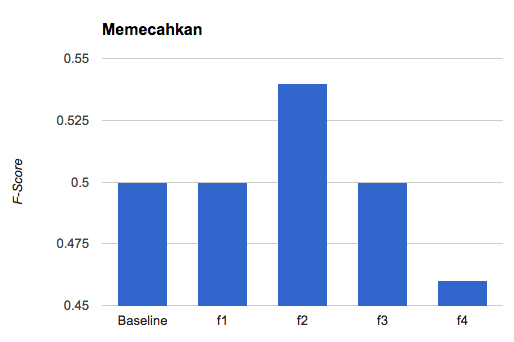
\includegraphics[width=1\linewidth]{adit_pics/memecahkan.png}
	\caption{Grafik evaluasi kata "memecahkan"}
	\label{fig:memecahkan}
\end{figure}

Kelas kata dari "memecahkan" dengan kamus \textit{crawling} berjumlah 4 buah yaitu:
\begin{lstlisting}
'split\%2:38:00::': 1, 'break\%2:30:03::': 5, 'resolve\%2:31:01::': 7, 'solve\%2:31:00::': 13
\end{lstlisting}
Kelas kata dari "memecahkan" dengan kamus \textit{bi-directional} berjumlah 3 buah yaitu:
\begin{lstlisting}
'break%2:30:03::': 5, 'resolve%2:31:01::': 7, 'solve%2:31:00::': 13
\end{lstlisting}

Pada kata "memecahkan" dapat dilihat bahwa performa sistem WSD menggunakan kamus \textit{crawling} sebagai \textit{alignment enhancement} mempunyai tingkat akurasi yang lebih tinggi untuk setiap fitur yang digunakan. Namun demikian, performa dengan fitur gabungan POS Tag dan \textit{bag of words} malah menurun jika dibandingkan dengan fitur \textit{word embedding} dan \textit{bag of words} saja, bahkan akurasi yang didapatkan di bawah baseline.

\subsection{\textit{Target word} "menolak"}

\begin{figure}
	\centering
	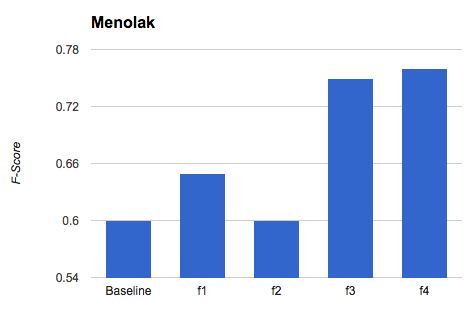
\includegraphics[width=1\linewidth]{adit_pics/menolak.png}
	\caption{Grafik evaluasi kata "menolak"}
	\label{fig:menolak}
\end{figure}


Kelas kata dari "menolak" dengan kamus \textit{crawling} berjumlah 9 buah yaitu:
\begin{lstlisting}
'rebuff%2:32:00::': 2, 'balk%2:41:00::': 3, 'object%2:32:00::': 1, 'dismiss%2:32:02::': 6, 'reject%2:40:00::': 82, 'refuse%1:27:00::': 1, 'oppose%2:32:01::': 10, 'resist%2:42:01::': 6, 'decline%2:32:00::': 198
\end{lstlisting}
Kelas kata dari "menolak" dengan kamus \textit{bi-directional} berjumlah 12 buah yaitu:
\begin{lstlisting}
'deny%2:32:00::': 6, 'spurn%2:32:00::': 1, 'rebuff%2:32:00::': 2, 'balk%2:41:00::': 1, 'object%2:32:00::': 1, 'dismiss%2:32:02::': 7, 'reject%2:40:00::': 80, 'refuse%1:27:00::': 1, 'oppose%2:32:01::': 5, 'refusal%1:10:01::': 3, 'resist%2:42:01::': 6, 'decline%2:32:00::': 197
\end{lstlisting}

Percobaan fitur f3 dan f4 pada kata "menolak" memiliki peningkatan performa akurasi jika dibandingkan dengan f1 atau bahkan f2 (\textit{word embedding}). Semua fitur yang dicoba pada kata ini memiliki performa diatas baseline kecuali f2. Perbedaan antara akurasi dengan menggunakan kamus \textit{crawling} ataupun \textit{bi-directional} tidak terlalu berbeda.

\subsection{\textit{Target word} "Obat"}

\begin{figure}
	\centering
	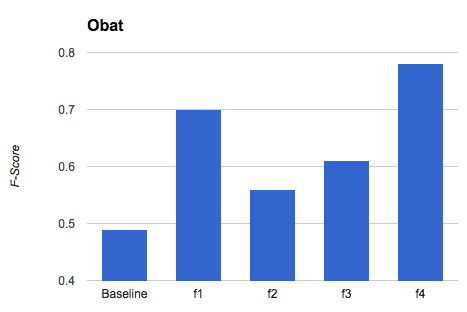
\includegraphics[width=1\linewidth]{adit_pics/obat.png}
	\caption{Grafik evaluasi kata "obat"}
	\label{fig:obat}
\end{figure}

Kelas kata dari "obat" dengan kamus \textit{crawling} berjumlah 2 buah yaitu:
\begin{lstlisting}
'medicine%1:09:00::': 48, 'drug%1:06:00::': 52, 
\end{lstlisting}
Kelas kata dari "obat" dengan kamus \textit{bi-directional} berjumlah 4 buah yaitu:
\begin{lstlisting}
'cure%1:06:00::': 7, 'medicine%1:09:00::': 46, 'drug%1:06:00::': 62, 'medication%1:06:00::': 22
\end{lstlisting}

Pada penggunaan kamus \textit{crawling}, semua fitur memiliki akurasi diatas baseline dan diatas performa penggunaan kamus \textit{bi-directional}. Dari kelas-kelas yang dihasilkan, dapat dilihat bahwa kamus \textit{crawling} hanya menghasilkan dua buah kelas makna kata untuk "obat", hal ini memungkinkan model untuk dapat menebak lebih akurat dari pada kasus ketika kelas makna kata lebih banyak.

\subsection{\textit{Target word} "Lingkungan"}

\begin{figure}
	\centering
	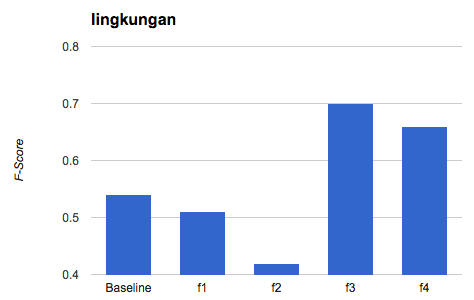
\includegraphics[width=1\linewidth]{adit_pics/lingkungan.png}
	\caption{Grafik evaluasi kata "lingkungan"}
	\label{fig:halaman}
\end{figure}

Kelas kata dari "lingkungan" dengan kamus \textit{crawling} berjumlah 7 buah yaitu:
\begin{lstlisting}
'environmentally%4:02:00::': 6, 'sphere%1:15:00::': 2, 'neighborhood%1:14:00::': 22, 'surroundings%1:15:00::': 1, 'environmental%3:01:01::': 72, 'environment%1:26:00::': 113, 'outside%5:00:00:external:00': 1
\end{lstlisting}
Kelas kata dari "lingkungan" dengan kamus \textit{bi-directional} berjumlah 7 buah yaitu:
\begin{lstlisting}
'environmentalist%1:18:00::': 1, 'sphere%1:15:00::': 2, 'neighborhood%1:14:00::': 22, 'environmental%3:01:01::': 74, 'vicinity%1:15:00::': 2, 'environment%1:26:00::': 113, 'outside%5:00:00:external:00': 1
\end{lstlisting}


Pada kata "lingkungan" hasil performa dengan penggunaan kamus \textit{crawling} memiliki performa lebih baik untuk semua fitur dibandingkan dengan \textit{bi-directional} walaupun kelas makna kata yang didapatkan dari dua buah kamus memiliki jumlah yang sama.

\subsection{\textit{Target word} "Halaman"}

\begin{figure}
	\centering
	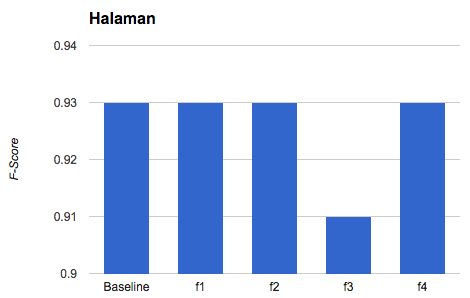
\includegraphics[width=1\linewidth]{adit_pics/halaman.png}
	\caption{Grafik evaluasi kata "halaman"}
	\label{fig:halaman}
\end{figure}

Kelas kata "halaman" dari hasil kamus \textit{crawling} memiliki 3 buah kelas yaitu:
\begin{lstlisting}
'page%1:10:00::': 41, 'yard%1:23:00::': 3, 'courtyard%1:06:00::': 3
\end{lstlisting}
Kelas kata dari "halaman" dengan kamus \textit{bi-directional} berjumlah 5 buah yaitu:
\begin{lstlisting}
'page%1:10:00::': 41, 'compound%1:09:00::': 1, 'yard%1:23:00::': 3, 'lawn%1:15:00::': 3, 'courtyard%1:06:00::': 3
\end{lstlisting}

Jumlah kelas pada kata "halaman" pada kedua buah skenario kamus sama-sama 3 buah dan performa yang dihasilkan oleh sistem yang menggunakan kamus \textit{crawling} mengungguli akurasi dari kamus \textit{bi-directional}. Fitur pada kedua skenario sama-sama turun pada f3 (POS Tag) dan meningkat pada fitur gabungan (f4).

\subsection{\textit{Target word} "Kehadiran"}

\begin{figure}
	\centering
	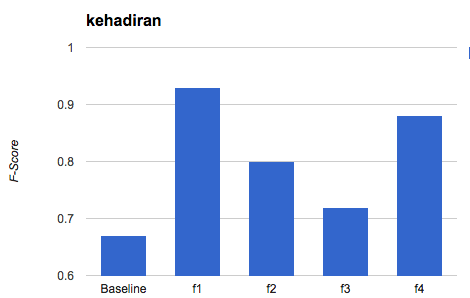
\includegraphics[width=1\linewidth]{adit_pics/kehadiran.png}
	\caption{Grafik evaluasi kata "kehadiran"}
	\label{fig:kehadiran}
\end{figure}

Kelas kata "kehadiran" dari hasil kamus \textit{crawling} memiliki 3 buah kelas yaitu:
\begin{lstlisting}
'attendance%1:04:00::': 19, 'presence%1:09:00::': 64, 'existence%1:26:00::': 1
\end{lstlisting}
Kelas kata dari "kehadiran" dengan kamus \textit{bi-directional} berjumlah 6 buah yaitu:
\begin{lstlisting}
'arrive%2:38:00::': 1, 'presence%1:09:00::': 64, 'attendance%1:04:00::': 18, 'prevent%2:41:01::': 1, 'teacher%1:18:00::': 2, 'participation%1:04:00::': 3
\end{lstlisting}

Kata "kehadiran" dengan kamus \textit{crawling} memiliki performa lebih baik dari setiap fitur dengan kamus \textit{bi-directional}. Berdasarkan jumlah kelas kata masing-masing skenario (kamus), \textit{bi-directional} menghasilkan jumlah kelas kata yang lebih banyak sehingga kemungkinan menyebabkan \textit{classifier} melakukan klasifikasi yang lebih sulit dari pada \textit{crawling based dictionary}.

\subsection{\textit{Target word} "Hati"}

\begin{figure}
	\centering
	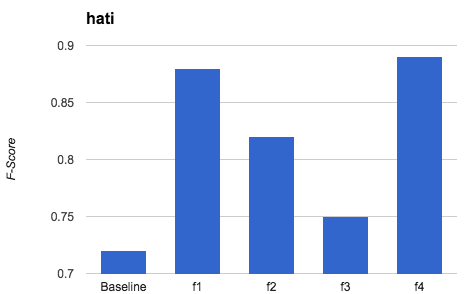
\includegraphics[width=1\linewidth]{adit_pics/hati.png}
	\caption{Grafik evaluasi kata "hati"}
	\label{fig:hati}
\end{figure}

Kelas kata "hati" dari hasil kamus \textit{crawling} memiliki 3 buah kelas yaitu:
\begin{lstlisting}
'liver%1:08:00::': 44, 'heart%1:09:00::': 170, 'mind%1:09:00::': 7
\end{lstlisting}
Kelas kata dari "hati" dengan kamus \textit{bi-directional} berjumlah 3 buah yaitu:
\begin{lstlisting}
'liver%1:08:00::': 44, 'heart%1:09:00::': 176, 'humble%5:00:00:inferior:01': 1
\end{lstlisting}

Pada kasus kata "hati", performa sistem dengan kamus \textit{bi-directional} menungguli setiap fitur jika dibandingkan dengan kamus \textit{crawling}. Kedua buah skenario kamus memiliki pola yang sama yaitu menungguli baseline pada f1, turun pada saat menggunakan f2 dan f3, dan akhirnya naik kembali akurasinya pada fitur f4. 

\subsection{\textit{Target word} "Coklat"}

\begin{figure}
	\centering
	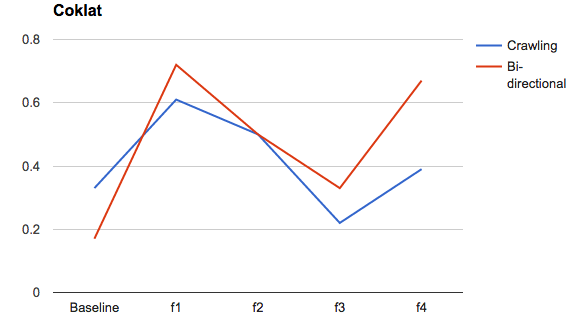
\includegraphics[width=1\linewidth]{adit_pics/coklat.png}
	\caption{Grafik evaluasi kata "coklat"}
	\label{fig:coklat}
\end{figure}

Kelas kata "coklat" dari hasil kamus \textit{crawling} memiliki 3 buah kelas yaitu:
\begin{lstlisting}
'cocoa%1:13:02::': 10, 'cacao%1:20:00::': 5, 'brown%5:00:00:chromatic:00': 4
\end{lstlisting}
Kelas kata dari "coklat" dengan kamus \textit{bi-directional} berjumlah 3 buah yaitu:
\begin{lstlisting}
'cocoa%1:13:02::': 11, 'cacao%1:20:00::': 5, 'brown%5:00:00:chromatic:00': 4
\end{lstlisting}

Kelas makna kata pada kedua skenario kamus sangatlah mirip dan hanya berbeda satu buah \textit{instance} lebih pada makna 'cocoa'. Dengan data yang lebih banyak pada skenario kamus \textit{bi-directional}, akurasi yang dihasilkan oleh sistem lebih baik dari \textit{crawling based} walaupun hanya lebih banyak satu buah data.

\subsection{\textit{Target word} "Berat"}

\begin{figure}
	\centering
	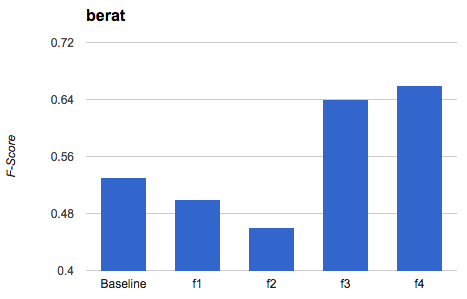
\includegraphics[width=1\linewidth]{adit_pics/berat.png}
	\caption{Grafik evaluasi kata "berat"}
	\label{fig:berat}
\end{figure}

Kelas kata "berat" dari hasil kamus \textit{crawling} memiliki 10 buah kelas yaitu:
\begin{lstlisting}
'heavily%4:02:00::': 3, 'tough%3:00:03::': 15, 'hard%4:02:00::': 1, 'weigh%2:42:01::': 8, 'heavy%3:00:04::': 58, 'weight%1:07:00::': 26, 'hard%5:00:00:strong:00': 3, 'difficult%3:00:00::': 8, 'strenuous%5:00:00:energetic:00': 2, 'severe%5:00:02:nonindulgent:00': 4
\end{lstlisting}
Kelas kata dari "berat" dengan kamus \textit{bi-directional} berjumlah 10 buah yaitu:
\begin{lstlisting}
'tough%3:00:03::': 15, 'hard%4:02:00::': 1, 'weigh%2:42:01::': 10, 'heavy%3:00:04::': 58, 'weight%1:07:00::': 26, 'hard%5:00:00:strong:00': 3, 'difficult%3:00:00::': 9, 'challenging%5:00:00:difficult:00': 1, 'violent%3:00:00::': 1, 'severe%5:00:02:nonindulgent:00': 4
\end{lstlisting}

Performa sistem dengan dua buah skenario kamus pada kata "berat" memiliki akurasi yang sama pada fitur f2 dan f3. Pada fitur kombinasi (f4), kedua sistem memiliki akurasi diatas baseline dan diungguli oleh sistem dengan kamus hasil \textit{crawling}.

\subsection{\textit{Target word} "Jalan"}

\begin{figure}
	\centering
	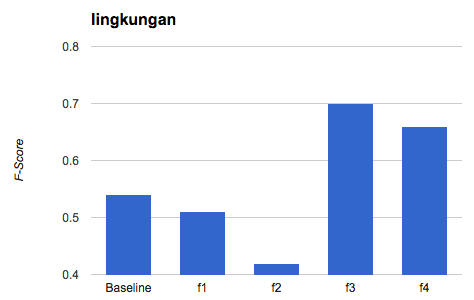
\includegraphics[width=1\linewidth]{adit_pics/lingkungan.png}
	\caption{Grafik evaluasi kata "jalan"}
	\label{fig:jalan}
\end{figure}

Kelas kata "jalan" dari hasil kamus \textit{crawling} memiliki 10 buah kelas yaitu:
\begin{lstlisting}
'way%1:15:00::': 106, 'path%1:04:00::': 13, 'street%1:06:00::': 45, 'highway%1:06:00::': 4, 'recourse%1:04:00::': 1, 'road%1:06:00::': 347, 'walkway%1:06:00::': 1
\end{lstlisting}
Kelas kata dari "jalan" dengan kamus \textit{bi-directional} berjumlah 14 buah yaitu:
\begin{lstlisting}
'go%2:30:02::': 3, 'way%1:15:00::': 101, 'traffic%1:14:00::': 3, 'pursue%2:38:00::': 1, 'highway%1:06:00::': 4, 'walk%1:04:01::': 2, 'option%1:21:00::': 1, 'move%2:41:01::': 2, 'passage%1:04:01::': 5, 'road%1:06:00::': 344, 'walk%2:33:00::': 2, 'choice%1:09:00::': 1, 'street%1:06:00::': 44, 'path%1:04:00::': 11
\end{lstlisting}

Performa pada kedua buah skenario tidak berbeda jauh dan diungguli oleh kamus \textit{bi-directional}. Jumlah makna kelas kata dengan kamus \textit{bi-directional} memiliki 14 buah kelas yang mana lebih banyak dari sistem dengan kamus \textit{crawling}. Walaupun memiliki jumlah kelas makna kata yang lebih banyak, sistem dengan kamsu \textit{bi-directional} memiliki performa yang lebih baik yang mungkin dikarenakan data yang lebih banyak.

Berdasarkan berbagai grafik dari masing-masing kata \textit{sample}, fitur yang biasanya mengalami penurunan adalah dari fitur f1 ke f2. Walaupun f2 merupakan fitur yang memanfaatkan model \textit{word embedding}, sepertinya perbedaan antara \textit{training} data yang digunakan untuk model ini memengaruhi performa dari penggunaan fitur ini pada \textit{classifier}. Data \textit{training} yang digunakan untuk \textit{word embedding} berasal dari Wikipedia dengan bentuk dan struktur kalimat/kata domain ensiklopedia sementara kalimat dalam korpus identik memiliki struktur \textit{general} domain yang di dalamnya terdapat kalimat-kalimat domain berita, obrolan sehari-hari, dan lain-lain. Perbedaan inilah yang memungkinkan kurang optimalnya fitur \textit{word embedding} dalam melakukan WSD pada penelitian ini. Pada fitur lain yaitu f4, dapat dilihat bahwa performa yang dihasilkan dengan gabungan fitur ini (POS Tag dan \textit{bag of words}) menghasilkan peningkatan ataupun juga penurunan pada beberapa kasus kata. Berdasarkan data tersebut, dapat disimpulkan juga bahwa performa fitur f1 dan f4 dapat mengungguli baseline pada banyak contoh kasus kata tersebut dengan total minimal delapan buah kata yang memiliki performa f1 atau f4 diatas baseline.